% ferry_paper.tex: GENERATED by DeveloperDocs/paper/assemble.py from front.tex,
% methods.tex, setup.tex, evaluation.tex, back.tex and results/exp5/paper/*.tex.
% Edit those sources and rerun the script; edits here are overwritten.
% =============================================================================
% Front matter of the FeRRy paper: preamble, title, abstract, introduction,
% Table 1 and related works. Extracted on 8 Oct 2026 from Hermes_paper (6).tex
% (the live text only; commented and \iffalse'd drafts dropped), with a revised
% introduction. DeveloperDocs/paper/assemble.py appends methods.tex,
% evaluation.tex and back.tex to this file to build ferry_paper.tex.
% =============================================================================
\documentclass[conference]{IEEEtran}
\IEEEoverridecommandlockouts

% Text, Language, and URLs
\usepackage[utf8]{inputenc}
\usepackage[english]{babel}
\usepackage[hyphens]{url}
\usepackage{cite}

% Math and Symbols
\usepackage{amsmath,amssymb,amsfonts} % amssymb is included here
\usepackage{textcomp}

% Figures, Subfigures, and Colors
\usepackage{float}
\usepackage{graphicx}
\usepackage{subcaption}
\usepackage[table]{xcolor} % Updated to include [table] option

% Tables and Formatting
\usepackage{multirow}
\usepackage{tabularx}
\usepackage{booktabs} % Already existed
\usepackage{makecell} % Already existed
\usepackage{diagbox}
\usepackage{multicol}
\usepackage{fancyhdr}
\usepackage{colortbl} % Added for cell coloring
\usepackage{array}    % Added for advanced array/table options

% Custom Table Columns
\newcolumntype{L}{>{\raggedright\arraybackslash}X}
\newcolumntype{P}[1]{>{\centering\arraybackslash}m{#1}}

% Algorithms (Using algorithm + algpseudocode exclusively to avoid conflicts)
\usepackage{algorithm}
\usepackage{algpseudocode}

% TikZ and PGFPlots
\usepackage{tikz}
\usetikzlibrary{positioning, arrows.meta, calc}
\usepackage{pgfplots}
\pgfplotsset{compat=1.18} 

% Custom command definitions (defined exactly once)
\newcommand{\threat}[1]{\text{#1}}
\newcommand{\securitymechanism}[1]{\mathcal{S}_{\text{#1}}}
\newcommand{\protocol}[1]{\mathcal{C}_{\text{#1}}}
\newcommand{\experiment}[1]{\mathcal{E}_{\text{#1}}}
\newcommand{\performance}[1]{P_{\text{#1}}}

% FeRRy macros (methods and evaluation)
\newcommand{\sysname}{FeRRy}
\newcommand{\bbar}{\bar{b}}
\newcommand{\Tnom}{T_{\mathrm{nom}}}

\pagestyle{plain}

% \def\BibTeX{{\rm B\kern-.05em{\sc i\kern-.025em b}\kern-.08em
%     T\kern-.1667em\lower.7ex\hbox{E}\kern-.125emX}}


\makeatletter
\newcommand{\linebreakand}{%
  \end{@IEEEauthorhalign}
  \hfill\mbox{}\par
  \mbox{}\hfill\begin{@IEEEauthorhalign}
}
\makeatother

\begin{document}
% TODO(title): the paper now presents FeRRy; the old title named HERMES.
\title{FeRRy: RF-Aware Mission Planning for Federated Learning with Drones as Data Mules}
% Authors: omitted for double-anonymous review. The \author block (names,
% affiliations, emails) is kept in the Overleaf copy, not in this public repo;
% restore it there for the camera-ready.

\maketitle

% Abstract: the short hybrid of abstract_revision.md, adopted 8 Oct 2026
% (the document keeps the earlier versions and the audit of the original).
\begin{abstract}
Federated learning (FL) supports privacy by letting devices train a shared model
without sharing their raw data, but assumes every device can reach a central
server. In contested and disaster-zone deployments that assumption fails:
devices that are out of range or poorly connected are skipped repeatedly, and
federation rounds stall. Unmanned aerial vehicles (UAVs) acting as data mules can
carry model updates to and from such devices, but a mule has a finite mission
budget, and its radio decides how far it reaches. We present FeRRy, a
Federated RF-aware Routing framework that treats a mule's reach as a decision,
through three components. First, before each flight, a band-aware mission planner
chooses the contact band class, which trades range for rate, together with the
route, under one feasibility test of per-device deadlines and the mission budget,
with a coverage term that keeps devices from being starved. Second, in flight,
the mule re-plans the rest of its route when the observed channel uses up the
plan's slack, and a per-stop rule can switch to a faster band and reorder the
remaining stops, each reorder checked by the same test. Third, a hierarchical
aggregation layer merges updates on each mule, then across mules at the edge
server, weighting stale updates down. In a prototype whose server, mules and
devices run as separate processes over TCP and train a real intrusion-detection
model on CICIoT2023, with flight time, the radio channel and energy simulated, we
compare FeRRy with seven baseline schedulers, including adaptations of
mobile-transporter federated learning (FedEx), Oort, FedCS and a Whittle-index
age-of-update scheduler. With six devices, one mule and a moderate budget, FeRRy
reaches the target accuracy 27--31\% sooner than each baseline, because its plan
chooses a long-reach narrow band that removes most of the transit between stops.
Under tight budgets, it keeps the age of updates about a quarter lower than
age-of-information schedulers and, with 24 devices, reaches the target 12\%
sooner than FedEx's route. Its plans stay within a tight budget in 70\% of
missions, overrunning by only 8.5\,s on average otherwise.
\end{abstract}

\begin{IEEEkeywords}
Decentralized learning, federated learning, UAV data mules, tactical edge computing, mobile relay networks
\end{IEEEkeywords}

\section{Introduction}
\label{sec:introduction}

Disaster response, wildfire monitoring, agricultural sensing and tactical
operations increasingly rely on edge devices deployed where fixed infrastructure
is sparse, damaged or absent~\cite{zeng2016wireless, song2022comprehensive}.
These are also the settings most prone to denied, disrupted, intermittent and
limited (DDIL) connectivity~\cite{gupta2015survey}. Federated learning (FL) suits
them, because devices exchange model updates rather than raw
data~\cite{mcmahan2017communication, kostage2025hifins}, but it still needs every
device to reach the server: when a device cannot, its update is lost, and rounds
close short, time out, or fail to produce a usable model~\cite{li2020federated}.
The gap is not faster FL communication but federation that continues when the
network itself is fragmented.

UAVs acting as data mules can bridge disconnected regions by carrying model state
between devices and servers~\cite{zhang2025latency, arsalaan2024uavs}, but a mule
has limited flight time and energy, and a contact is useful only if an update is
ready and the link can sustain the transfer when the mule arrives. Hierarchical
FL, UAV-assisted FL, physical model transport, RF-adaptive networking and client
selection each address part of this problem~\cite{liu2020client, lin2023delay,
parasnis2023connectivity, yemini2023robust, mestoukirdi2022uav, bian2025indirect,
wang2018deep, cui2019multi, nishio2019client, lai2021oort}, but they retain
persistent reachability, stationary aggregation, or a communication setting that
the mobility decision does not control.

We present \sysname{}, a Federated RF-aware Routing framework whose central
observation is that a mule's radio reach is itself a decision. A contact band
with a narrower occupied bandwidth reaches farther at a lower rate: it can serve
a whole field from one stop at the cost of a longer dwell, whereas a wide band
serves each device quickly but only from nearby, so the mule spends most of its
mission in transit. Which trade wins depends on how many devices need service,
where they are and how much time remains, so \sysname{} chooses the band class
and the route together, before each flight.

\sysname{} decides on two clocks. On the \emph{plan clock}, at the dock, it
searches band classes and routes under one feasibility test of per-device
deadlines and the mission budget, and commits the plan that serves the most
coverage weight, a weight that grows with the missions since a device last
contributed. On the \emph{flight clock}, a per-stop rule can use the observed
channel to pick a faster band or reorder the remaining stops, and the mule
re-plans when the channel has used up the plan's slack. Updates are merged on
the mule with staleness weights and across mules at the server, so rounds close
with what arrives. We evaluate three variants: F commits the plan, FX adds a
fixed per-stop rule, and FQ a learned one.

In a multi-process prototype that trains a real intrusion-detection model on
CICIoT2023~\cite{CiCIoT2023}, with mission time, the channel and energy
simulated, we compare \sysname{} with seven whole schedulers under a
pre-registered analysis plan. With six devices and one mule, it reaches the
target accuracy 27--31\% sooner than each, because its plan chooses the
long-reach narrow band and cuts the transit between stops from about 140\,s to
15\,s; pinned to the wide band, it is no faster than FedEx's route. Under tight
budgets it keeps updates fresher than age-of-information schedulers. Learning
adds nothing to the fixed per-stop rule, and an exploratory comparison locates
the gain in the plan: inside it, the learned score reaches the target 36\%
sooner than a learned scheduler without one. We also report \sysname{}'s limits:
its plan prices the mean channel, so it overruns tight budgets in 30\% of
missions, and it does not price training time.

The contributions of this paper are:

\begin{itemize}

\item \textbf{Reach as a mission decision.} We treat the contact band class,
which sets how far a mule reaches and how fast it transfers, as a decision made
jointly with the route under a mission budget, and give a planner that searches
both under one feasibility test.

\item \textbf{A two-clock design with bounded learning.} The same test gates a
dock-time plan and in-flight per-stop decisions, with adaptive per-device
deadlines, a coverage weight and age cap against starvation, and
staleness-weighted merges; learning ranks only what the gates admit.

\item \textbf{A prototype and a simulator built from the same code.} A
multi-process prototype that trains a real model, and FerrySim, which trains the
learned components and plans for up to 96 devices.

\item \textbf{A pre-registered comparison with the state of the art.} Against
seven whole schedulers, on paired seeds with multiplicity correction, we report
where \sysname{} wins, why, which parts of its design have no measurable effect,
and where it falls short.

\end{itemize}

Section~\ref{sec:related_works} reviews related work,
Section~\ref{sec:method} presents \sysname{}'s design,
Section~\ref{sec:setup} the experimental setup and design,
Section~\ref{sec:results} the results, and Section~\ref{sec:conclusion}
concludes.

\definecolor{goodgreen}{RGB}{178,210,150}
\definecolor{ferrygreen}{RGB}{105,160,90}
\definecolor{badred}{RGB}{230,170,160}
\definecolor{nayellow}{RGB}{240,210,120}

\newcommand{\cmarkc}{\cellcolor{goodgreen}\textcolor{black!55}{\scriptsize$\checkmark$}}
\newcommand{\xmarkc}{\cellcolor{badred}\textcolor{black!40}{\scriptsize$\times$}}
\newcommand{\tmarkc}{\cellcolor{nayellow}\textcolor{black!65}{\scriptsize$\triangle$}}
\newcommand{\cmarkF}{\cellcolor{ferrygreen}\textcolor{white}{\textbf{\scriptsize$\checkmark$}}}

\begin{table*}[!t]
\caption{\small \textsc{Comparison of Related FL, UAV Mobility, and RF-Aware Coordination Approaches}}
\label{tab:ferry-comparison}
\centering
\resizebox{\textwidth}{!}{%
\begin{tabular}{l c c c c c c}
\toprule
\multicolumn{1}{c}{Framework}
&
\begin{tabular}[c]{@{}c@{}}Physical Model\\ Transport\end{tabular}
&
\begin{tabular}[c]{@{}c@{}}Explicit RF\\ Decision\end{tabular}
&
\begin{tabular}[c]{@{}c@{}}Mobility / Route\\ Decision\end{tabular}
&
\begin{tabular}[c]{@{}c@{}}Deadline /\\ Freshness Aware\end{tabular}
&
\begin{tabular}[c]{@{}c@{}}In-Mission\\ Replanning\end{tabular}
&
\begin{tabular}[c]{@{}c@{}}Joint FL--Mobility/RF\\ Coordination\end{tabular}
\\
\midrule

Hierarchical FL
{\scriptsize \cite{liu2020client}}
& \xmarkc & \xmarkc & \xmarkc & \xmarkc & \xmarkc & \xmarkc \\

Delay-Aware HFL
{\scriptsize \cite{lin2023delay}}
& \xmarkc & \xmarkc & \xmarkc & \tmarkc & \xmarkc & \xmarkc \\

FedCS
{\scriptsize \cite{nishio2019client}}
& \xmarkc & \xmarkc & \xmarkc & \cmarkc & \xmarkc & \xmarkc \\

Oort
{\scriptsize \cite{lai2021oort}}
& \xmarkc & \xmarkc & \xmarkc & \cmarkc & \xmarkc & \xmarkc \\

UAV Multi-Community FL
{\scriptsize \cite{mestoukirdi2022uav}}
& \xmarkc & \xmarkc & \cmarkc & \tmarkc & \xmarkc & \cmarkc \\

FedEx
{\scriptsize \cite{bian2025indirect}}
& \cmarkc & \xmarkc & \cmarkc & \tmarkc & \xmarkc & \cmarkc \\

Model-Aided Multi-UAV RL
{\scriptsize \cite{chen2023model}}
& \xmarkc & \tmarkc & \cmarkc & \xmarkc & \cmarkc & \xmarkc \\

Deadline-Sensitive Multi-UAV
{\scriptsize \cite{mondal2025deep}}
& \xmarkc & \tmarkc & \cmarkc & \cmarkc & \cmarkc & \xmarkc \\

DRL Multichannel Access
{\scriptsize \cite{wang2018deep}}
& \xmarkc & \cmarkc & \xmarkc & \xmarkc & \xmarkc & \xmarkc \\

MARL UAV Resource Allocation
{\scriptsize \cite{cui2019multi}}
& \xmarkc & \cmarkc & \tmarkc & \xmarkc & \xmarkc & \xmarkc \\

Value-Aware UAV FL
{\scriptsize \cite{cui2023data}}
& \xmarkc & \xmarkc & \xmarkc & \cmarkc & \xmarkc & \xmarkc \\

UAV-Enabled Asynchronous FL
{\scriptsize \cite{zhai2024uav}}
& \xmarkc & \tmarkc & \cmarkc & \cmarkc & \xmarkc & \cmarkc \\

FedBuff
{\scriptsize \cite{nguyen2022federated}}
& \xmarkc & \xmarkc & \xmarkc & \cmarkc & \xmarkc & \xmarkc \\

Async-HFL
{\scriptsize \cite{yu2023async}}
& \xmarkc & \xmarkc & \xmarkc & \cmarkc & \xmarkc & \xmarkc \\

\midrule

\textbf{FeRRy (ours)}
& \cmarkF
& \cmarkF
& \cmarkF
& \cmarkF
& \cmarkF
& \cmarkF \\

\bottomrule
\end{tabular}%
}

\vspace{2pt}
{\footnotesize
\cmarkc\ Present
\quad
\xmarkc\ Absent
\quad
\tmarkc\ Partial / indirect
}
\end{table*}


% Architecture figure: OUT of the build (8 Oct 2026). The drawing,
% HERMES_Case_Scenarios_compact.drawio, is the HERMES design: "WITH HERMES"
% labels, a DDQN choosing among carrier frequencies (FeRRy's band classes share
% one carrier and differ in bandwidth; nothing in FeRRy's RF layer is learned),
% and the old gated job scheduler. Redraw it to match Section III (plan clock,
% flight clock, merges), then uncomment this block and restore
% "A cluster (Fig.~\ref{fig:architecture})" in methods.tex's Setting paragraph.
% \begin{figure*}[t]
%     \centering
%     \includegraphics[trim=0cm 0cm 0cm 0cm, clip, scale=0.35]{Figures/HERMES_Case_Scenarios_compact.drawio.png}
%     \caption{\sysname{} overview: field devices, UAV data mules, and the edge server.}
%     \label{fig:architecture}
% \end{figure*}

\section{Related Works}
\label{sec:related_works}

Federated learning reduces centralized data movement by allowing participants to train locally and exchange model updates rather than raw datasets. FedAvg established this model-averaging paradigm, while FedProx improved robustness to statistical and systems heterogeneity \cite{mcmahan2017communication,li2020federated}. Hierarchical approaches subsequently introduced intermediate aggregation to reduce communication cost and accommodate heterogeneous edge environments. Aggregation-oriented hierarchical FL performs partial aggregation at edge servers before cloud synchronization, while delay-aware hierarchical FL explicitly accounts for communication delay between edge and cloud tiers \cite{liu2020client,lin2023delay}. Connectivity-aware semi-decentralized FL further exploits time-varying device-to-device links, and collaborative relaying allows well-connected clients to forward updates for clients experiencing intermittent server connectivity \cite{parasnis2023connectivity,yemini2023robust}. These approaches improve FL under unreliable communication, but they still rely on a communication graph in which model state is eventually forwarded through wireless links. FeRRy targets the more disruptive case in which such an end-to-end path may not exist and model state must instead be physically transported between isolated participants.

UAV-assisted FL introduces mobility into the learning infrastructure, but the role assigned to the UAV varies considerably. A UAV may operate as a mobile FL server whose routing is optimized with bandwidth, computation, and transmit power \cite{zhang2025latency}, or as a mobile orchestrator that visits discrete locations while optimizing routing and device scheduling altogether across multiple FL communities \cite{mestoukirdi2022uav}.  These systems use mobility to restore or improve communication between ground participants and the learning infrastructure. The closest architectural precedent to FeRRy is FedEx, which removes direct client-server connectivity and uses mobile transporters to physically carry model information \cite{bian2025indirect}. FedEx establishes physical model transport and relates FL performance to transporter travel time, but assumes preplanned tours and fixed communication conditions without adapting service to changing RF conditions, per-device deadlines, or in-mission contact opportunities. FeRRy extends this setting by treating reachability, service time, participant urgency, and communication conditions as part of the mission decision itself.

Another research direction studies UAV trajectory planning together with communication-aware data collection. Earlier formulations have demonstrated that trajectory and communication should not be optimized independently, and should jointly optimize multi-UAV trajectories, user scheduling, association, and transmit power for wireless service \cite{wu2018joint}, while more recent learning-based approaches move these decisions online. Multi-UAV controllers have used SNR, reachability, remaining device data, relative distance, and battery state to learn trajectories \cite{chen2023model}, and subsequent work has learned 3-D trajectories and device scheduling \cite{gao2024federated}, incorporated collection deadlines, link quality, and energy constraints through MAPPO \cite{mondal2025deep}, further optimized trajectory and task offloading under AoI, latency, and energy objectives \cite{wang2025joint}, and considered battery and interference constraints in federated-RL data collection \cite{kumar2026battery}. RF adaptation has likewise been studied through deep reinforcement learning for dynamic multichannel access \cite{wang2018deep} and multi-agent resource allocation over users, power levels, and subchannels in UAV networks \cite{cui2019multi}. These studies establish that communication-aware, and energy-aware multi-UAV trajectory learning is already well studied. FeRRy therefore does not claim RF-aware trajectory planning itself as novel, instead, its distinction is that the communication choice directly changes the feasibility and duration of transporting FL updates, while participant urgency determines which contact is worth serving next.

Client-selection and freshness-aware scheduling provides another part of this coordination problem. Existing methods select participants according to round deadlines and resource availability \cite{nishio2019client}, favor clients with higher training loss \cite{cho2022towards}, or use statistical utility and participation history observed in previous rounds \cite{lai2021oort}. This distinction between pre-selection and historical information is particularly important for physical data muling because isolated participants cannot continuously report their current state before the UAV reaches them. Related UAV-FL work has further balanced update age and data value under unstable connectivity \cite{cui2023data}, incorporated freshness into fairness-oriented scheduling \cite{zhu2024fairness}, required devices to be served within a bounded number of slots \cite{zhai2024uav}, and increased the priority of previously failed or unscheduled devices \cite{mestoukirdi2022uav}. These studies establish age-aware ranking and mechanisms to reduce starvation. FeRRy instead focuses on how these concerns interact with physical transport cost, where servicing an old or valuable update also requires flight time, contact time, sufficient radio reach, and remaining mission budget. 

Finally, asynchronous and hierarchical FL research addresses model-version mismatch when participant updates arrive at different times. Prior work has buffered asynchronous client updates before applying server-side aggregation, reducing sensitivity to individual stragglers while remaining compatible with secure aggregation \cite{nguyen2022federated}. Other hierarchical approaches perform asynchronous aggregation across both gateway and cloud tiers while jointly considering device selection and gateway association in heterogeneous IoT environments \cite{yu2023async}. These methods assume that updates are delivered through the network, whereas physical data muling introduces travel time as an additional source of staleness. FeRRy therefore treats aggregation as part of the mission lifecycle, where the same age and deadline information is used to determine whether a participant to be served also influences whether its transported update remains useful when the mule returns. The key distinction is thus the coupling of physical admission, service order, RF-dependent contact feasibility, and update freshness, rather than a new aggregation mechanism in isolation.

Table~\ref{tab:ferry-comparison} shows that prior work addresses individual parts of this problem, including FL-aware participant selection, freshness-aware scheduling, UAV trajectory planning, RF adaptation, and physical model transport. However, even the closest transporter-based approach does not address RF-dependent reach and service time with participant deadlines and in-mission route adaptation. FeRRy addresses this gap by using communication conditions, mobility, and FL-update urgency to plan and revise model transport under a finite mission budget.

\section{\sysname{} Methodology}
\label{sec:method}

\sysname{} flies an autonomous mule (UAV) between edge devices and an edge
server. We describe it by \emph{decision clock} rather than by layer, because
its two main decisions each span the radio, scheduling and learning layers.

% -----------------------------------------------------------------------------
\subsection{Setting, Layer Roles, and Decision Clocks}
\label{sec:method:roles}

\paragraph{Setting}
A cluster has one edge server, one or more mules, and static field devices whose
positions the server's registry holds. Each mule gets a disjoint slice
$\mathcal{M}$ of the registry for the trial; with $K>1$ mules the slices are
angular sectors around the shared dock, within one device of equal size, and the
mules fly concurrently. Devices train offline between visits, so a contact is
exchange only: the mule pushes the global model and pulls the device's prepared
update. In \textsc{Pass 1} of a mission the mule collects updates along a route,
merges them on board and docks to upload; the server merges across mules into
the next global model. In \textsc{Pass 2} the mule delivers that model to its
whole slice, which gives each later update a known basis version, and so an age.
A budget $T_{\mathrm{miss}}$ bounds Pass~1: the plan and every check in flight
require the predicted landing and upload within $T_{\mathrm{miss}}$ of takeoff.

\paragraph{Learning task}
The devices train a binary intrusion detector on CICIoT2023~\cite{CiCIoT2023}, a
multilayer perceptron trained for one local epoch per model received, on 20{,}000
balanced training flows split across them; a disjoint 6{,}000-flow test set
scores each new global model, stamped when its closing upload completes. A device
with no prepared update trains inside the contact, at no simulated cost. Every
transfer is priced as $S=1$~MB.

\paragraph{Layer roles and clocks}
Table~\ref{tab:layer-roles} gives each layer's role. Hard gates (eligibility, the
feasibility test, and the age cap) always run before any ranking, so a ranking
rule, learned or not, chooses only among options the gates admit. On the
\emph{plan clock}, once per mission at the dock, the mule chooses a contact band
class $\bbar$ and a route together, because the band class fixes the contact
range, the range fixes the stops, and the stops fix the route
(Fig.~\ref{fig:clocks}). On the \emph{flight clock}, in Pass~1, it can revise the
band and the next stop from the signal it observes, since interference varies
over about one leg. Rate sets dwell, dwell advances mission time, mission time
decides feasibility, and infeasibility triggers a re-plan. Learning can enter
only through the flight slot.

\begin{table}[t]
\centering
\caption{Role of each layer in the joint decisions.}
\label{tab:layer-roles}
\small
\begin{tabularx}{\columnwidth}{l l L}
\toprule
\textbf{Layer} & \textbf{Role} & \textbf{Supplies to the decisions} \\
\midrule
L1 RF link & prices & Range, rate, dwell, and SNR over time for each band class; backhaul carrier \\
L2 Scheduling & decides & Admission, band class $\bbar$, route, per-arrival (band, next stop), re-plan \\
L3 Federated learning & values & Merge weight, update age, coverage weight, cross-mule merge \\
\bottomrule
\end{tabularx}
\end{table}

\begin{figure}[t]
\centering
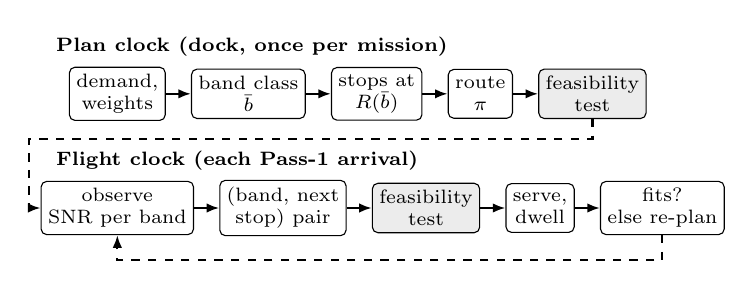
\begin{tikzpicture}[
  box/.style={draw, rounded corners=2pt, minimum height=0.62cm, align=center,
              font=\scriptsize, inner sep=2.5pt},
  gate/.style={box, fill=gray!15},
  arr/.style={-{Latex[length=1.6mm]}, thick},
  node distance=0.32cm]
  % plan clock
  \node[font=\scriptsize\bfseries, anchor=west] (pl) at (0,1.55) {Plan clock (dock, once per mission)};
  \node[box] (d) at (0.9,0.95) {demand,\\weights};
  \node[box, right=of d] (bb) {band class\\$\bbar$};
  \node[box, right=of bb] (st) {stops at\\$R(\bbar)$};
  \node[box, right=of st] (rt) {route\\$\pi$};
  \node[gate, right=of rt] (g1) {feasibility\\test};
  \draw[arr] (d)--(bb); \draw[arr] (bb)--(st); \draw[arr] (st)--(rt); \draw[arr] (rt)--(g1);
  % flight clock
  \node[font=\scriptsize\bfseries, anchor=west] (fl) at (0,0.1) {Flight clock (each Pass-1 arrival)};
  \node[box] (ob) at (0.9,-0.5) {observe\\SNR per band};
  \node[box, right=of ob] (pr) {(band, next\\stop) pair};
  \node[gate, right=of pr] (g2) {feasibility\\test};
  \node[box, right=of g2] (sv) {serve,\\dwell};
  \node[box, right=of sv] (rp) {fits?\\else re-plan};
  \draw[arr] (ob)--(pr); \draw[arr] (pr)--(g2); \draw[arr] (g2)--(sv); \draw[arr] (sv)--(rp);
  \draw[arr, dashed] (rp.south) -- ++(0,-0.32) -| (ob.south);
  \draw[arr, dashed] (g1.south) -- ++(0,-0.25) -| ($(ob.west)+(-0.15,0)$) -- (ob.west);
\end{tikzpicture}
\caption{The two decision clocks; the flight row shows FQ's per-stop choice.}
\label{fig:clocks}
\end{figure}

% -----------------------------------------------------------------------------
\subsection{Quantities Supplied by the Layers}
\label{sec:method:models}

\subsubsection{L1: Contact Link, Mission Time, and Backhaul}
\label{sec:method:l1}

\paragraph{Band classes}
The contact link offers three band classes $\mathcal{B}$ on one carrier, LTE
channel bandwidths~\cite{3gpp36104} with occupied bandwidth
$B_b=N_{\mathrm{RB}}\times180$~kHz: \textsf{wide} (20~MHz, 100 resource blocks),
\textsf{medium} (5~MHz, 25) and \textsf{narrow} (1.4~MHz, 6). With a common
transmit power and a noise floor that scales with $B_b$, a narrower class
reaches farther at a lower rate:
\begin{equation}
R_b^{3D} = R_0^{3D}\left(\frac{B_0}{B_b}\right)^{1/n},
\qquad
R_b = \sqrt{\left(R_b^{3D}\right)^2 - h^2},
\label{eq:range}
\end{equation}
relative to a reference class $(B_0,R_0^{3D})$, with path-loss exponent $n=2.2$
and altitude $h=25$~m. Anchoring \textsf{wide} at 60~m gives planar ranges of
60, 120 and 232~m, at which the mean SNR clears the decoding floor by a 5.1~dB
shadowing margin $M_{\mathrm{sh}}$ (reach probability 0.9 under shadowing).

\paragraph{Rate and dwell}
The mean SNR at distance $d$ is
$\bar\gamma_b(d)=\gamma_{\mathrm{floor}}+M_{\mathrm{sh}}+10\,n\log_{10}(R_b^{3D}/d^{3D})$,
with $\gamma_{\mathrm{floor}}=-6.7$~dB (CQI~1), and the rate is
\begin{equation}
r_b(\gamma)=\min\bigl\{\kappa_b B_b\,\mathrm{SE}(\gamma),\;B_b\log_2(1+10^{\gamma/10})\bigr\},
\label{eq:rate}
\end{equation}
for $\gamma\ge\gamma_{\mathrm{floor}}$ and zero below, with $\mathrm{SE}$ the CQI
spectral efficiency and $\kappa_b$ an implementation efficiency. Moving $S_j$
bytes takes $\tau_{j,b}^{\mathrm{dwell}}(\gamma)=8S_j/r_b(\gamma)$: $2S$ for a
Pass-1 session, $S$ for a delivery or the upload, with the dwells at a stop
adding up. The channel only decides whether a device is solicited (not if it is
below the floor on arrival) and how long its session takes; a started session
always completes, and the TCP messages carry no radio effects.

\paragraph{Channel over time}
The realized SNR of device $j$ on class $b$ at mission time $t$ is
\begin{equation}
\gamma_{b,j}(t)=\bar\gamma_b(d_j)+X_j(t)+A\sin\bigl(2\pi(t/P_c+\phi_b)\bigr)+\sigma_I\,\xi_b(t),
\label{eq:realsnr}
\end{equation}
with correlated shadowing $X_j$ ($\sigma_{\mathrm{sh}}=4$~dB, 7.4~s correlation
time) and per-class interference~\cite{3gpp36777} of period $P_c=60$~s, phases
$\phi_b\in\{0,\tfrac13,\tfrac23\}$ and noise $\xi_b$; the interference-limited
(``jittery'') regime sets $A=5$~dB and $\sigma_I=1.5$~dB. Keyed hashes give every
policy the same draws. The planner prices only the mean $\bar\gamma_b$, so
realized missions run longer than planned, and uses the outage probability
\begin{equation}
p_{\mathrm{out}}(b,d)=\Phi\!\left(\frac{\gamma_{\mathrm{floor}}-\bar\gamma_b(d)}{\sigma_{\mathrm{eff}}}\right),
\quad
\sigma_{\mathrm{eff}}^2=\sigma_{\mathrm{sh}}^2+\sigma_I^2+\tfrac{A^2}{2};
\label{eq:pout}
\end{equation}
the flight clock observes $\gamma_{b,j}(t)$.

\paragraph{Mission time and energy}
Mission time is simulated time since takeoff, charged for transit at 5~m/s,
dwell, a 1~s listen at a stop with a missing reply, the return, the upload and a
30~s dock turnaround. Propulsion energy follows the same ledger,
\begin{equation}
E = P_{\mathrm{move}}\,(t_{\mathrm{transit}}+t_{\mathrm{return}})
  + P_{\mathrm{hover}}\,(t_{\mathrm{dwell}}+t_{\mathrm{listen}}),
\label{eq:energy}
\end{equation}
with $P_{\mathrm{move}}=143.6$~W and $P_{\mathrm{hover}}=168.5$~W from Zeng et
al.'s rotary-wing model~\cite{zeng2019energy}; no battery limit is enforced.

\paragraph{Backhaul}
The upload rides the best of three backhaul carriers and is lost with probability
2\%, without retry: Pass~2 then delivers the unchanged model, and the planner,
which records the devices as merged before the upload, counts them as served.
The component ablations' backhaul test and the radio study
(Table~\ref{tab:studies}) use a time-varying backhaul instead, which loses about
a fifth of the uploads on the fixed carrier (F closes 79\% of its rounds,
against 97\%); only there does the adaptive carrier controller (F+L1) act, and
since it sees the SNR that decides each loss, it is close to an oracle. The
backhaul never enters a scheduling decision.

\subsubsection{L2/L3: Demand, Deadlines, Ages, and the Age Cap}
\label{sec:method:demand}

\paragraph{Contact outcomes}
A Pass-1 contact is \emph{clean} when the device returns an update with the
expected round, size and checksum, \emph{partial} when it answers but refuses
or fails those checks, and otherwise a \emph{timeout}. Whether a reachable device
replies is drawn each mission from its reliability $\rho_j\sim U(0.15,1)$; a lost
reply still costs the push. A session that outlasts its wall-clock timeout (36~s
at $N=6$) is a timeout; results were identical at 0.75 to 1.5 times that value.
A device can also be given a log-normal training time, restarted by each model
it receives; an update not ready on arrival is a timeout, and the plan does not
price training time.

\paragraph{Per-device deadline}
Each device $j$ has a fulfilment window $\Phi(j)$ and a deadline
\begin{equation}
\mathrm{Deadline}(j)=t+\Phi(j)-\iota(j),
\label{eq:deadline}
\end{equation}
with $t$ the planning time and $\iota(j)$ the time since its last clean contact.
After each contact the window is scaled and clamped,
\begin{equation}
\Phi(j)\leftarrow\min\{\Phi_{\max},\max\{\Phi_{\min},\,\beta_{o}\,\Phi(j)\}\},
\label{eq:phi}
\end{equation}
with $\beta_{\mathrm{clean}}=0.8$; $\beta_{\mathrm{partial}}=1.25$ for a partial
or a timeout after the device answered; and $\beta_{\mathrm{timeout}}=1.5$ for a
silent, unreachable or left-out device. In units of $\sigma=\Tnom/10$~s, where
$\Tnom$ is the median nominal two-pass mission on the wide band (203~s at $N=6$),
$\Phi_0=60\sigma$, $\Phi_{\min}=5\sigma$ and $\Phi_{\max}=300\sigma$~s. A clean
contact re-anchors $\iota(j)$; a failed one widens the window but leaves the
anchor stale, so a device that keeps failing grows more overdue. A device the
plan leaves out, or the mule drops in flight, counts as a timeout.

\paragraph{Ages and coverage weight}
The \emph{plan age} $a_j=m-U_j$ counts the missions since the mission $U_j$ whose
merge last used the device's update, and strengthens its claim to be served. The
\emph{merge age} $a_i=v-b_i$ of an update is the mule's model version minus the
version $b_i$ the device trained from, which it echoes; it discounts the update
in the merge. A miss relaxes a device's \emph{window} but not its
\emph{priority}, which enters through the coverage weight
\begin{equation}
w_j=\max(a_j,1)\,(1+\mu_j),
\label{eq:covweight}
\end{equation}
with $\mu_j$ the miss streak; under a plan, $\mu_j=a_j-1$, so $w_j\approx a_j^2$.

\paragraph{Age cap}
A device is \emph{capped} when $a_j\ge S$, with $S=2$ from a pilot (the fewest
missions that serve every servable device on 90\% of layouts at the stress
budget). A stop's deadline is the earliest among its uncapped members, and a
stop of capped members only is exempt from it but not from the budget; a trimmed
route flies stops with a capped member first; a capped device its stop cannot
serve within the budget gets a one-device \emph{hover stop}; and the plan key
first compares the ages of the capped devices a plan leaves out.

% -----------------------------------------------------------------------------
\subsection{The Feasibility Test}
\label{sec:method:gate}

One predicate decides whether a stop may be served next, and it is the only
admission rule: it checks the committed plan, the plan search, every departure,
the re-plan and the in-flight choices. For a stop $s$ with members
$\mathcal{M}_s$, reached from a state (pose, mission time $c$, energy) on band $b$,
\begin{align}
t_{\mathrm{arr}} &= c+\|\mathrm{pose}-s\|/v,\\
t_{\mathrm{fin}} &= t_{\mathrm{arr}}+\!\!\sum_{j\in\mathcal{M}_s}\!\tau^{\mathrm{dwell}}_{j,b}(\bar\gamma_b(d_j)),\\
t_{\mathrm{home}} &= t_{\mathrm{fin}}+t_{\mathrm{return}}+t_{\mathrm{upload}},
\end{align}
and the stop is admitted only if $t_{\mathrm{fin}}$ meets its deadline,
$t_{\mathrm{home}}$ falls within takeoff plus $T_{\mathrm{miss}}$, and the energy
of Eq.~\eqref{eq:energy} fits any capacity set. The clauses are monotone in the
member set, so a stop that fails whole can be reduced to the members that fit.
The departure check catches a stop that the realized channel lengthens, but
nothing re-checks after the last Pass-1 stop, so a mission can overrun.

% -----------------------------------------------------------------------------
\subsection{Plan Clock: Reach and Route}
\label{sec:method:plan}

At the dock the mule commits a plan $\mathcal{P}=(\bbar,\pi)$: the band class for
both passes and an ordered list of stops, each reduced to the members that fit.

\paragraph{Reach is a decision}
For each class, a greedy anchor sweep clusters the slice into stops at the range
$R_b$. A wide class serves few devices per stop at a high rate; a narrow class
can reach the field from one stop but dwells longer. No fixed rule chooses
between them, so the planner prices every class and commits the best.

\paragraph{Route search}
Routes pass the feasibility test stop by stop. Up to six devices, an exact search
enumerates every ordered sequence of stops and member subsets and is optimal over
what the score prices; with up to six stops, it searches ordered stop subsets;
beyond that, a deterministic local search (2-OPT, then first-improvement moves,
at most 2000 evaluations per class) runs. The empty plan is chosen only if no
other is admitted.

\paragraph{Plan score and plan key}
Candidates are scored by
\begin{equation}
V(\bbar,\pi)=-\Bigl[c_1\Bigl(\tfrac{\Delta}{\Tnom}\Bigr)^{2}+c_2U+c_3L+c_4\frac{E}{P_{\mathrm{hover}}\Tnom}\Bigr],
\label{eq:planscore}
\end{equation}
with $\Delta$ the duration of the two-pass mission on $\bbar$, $E$ its energy, and
\begin{equation}
U=1-\frac{\sum_{\text{served}}w_j}{\sum_{\text{demand}}w_j},
\qquad
L=\frac{\sum_{\text{served}}w_j\,p_{\mathrm{out}}(\bbar,d_j)}{\sum_{\text{demand}}w_j}
\end{equation}
the weighted coverage shortfall and expected link loss ($c_1=1$,
$c_2=c_3=N_{\mathrm{demand}}$, $c_4=0.1$). The form follows FedEx's
route-dependent bound~\cite{bian2025indirect}, but the constants are hand-set and
the term in $\Delta$ is a staleness surrogate. Since every non-empty plan pays
for a whole Pass~2, $V$ alone can prefer to fly empty, so the mule commits the
plan with the smallest key
\begin{equation}
\bigl(\kappa_{\mathrm{cap}},\;-\textstyle\sum_{\text{served}}w_j/\sum_{\text{demand}}w_j,\;-V,\;\text{class index}\bigr),
\label{eq:plankey}
\end{equation}
compared lexicographically, with $\kappa_{\mathrm{cap}}$ the ages of the capped
devices the plan leaves out, largest first: time and energy break ties among
plans that serve the same weight. A guard fold re-checks the route before
commit, and every device left out is recorded as a miss.

% -----------------------------------------------------------------------------
\subsection{Flight Clock: Band, Next Stop, and Re-Planning}
\label{sec:method:flight}

\paragraph{The flight slot}
In Pass~1 the mule can revise, per stop, the band on which to serve the stop it
has reached and the next stop of the queue. F, the reference arm, leaves the
slot empty and flies the plan's band and order. The fixed filling, FX, picks on
arrival the fastest class that still reaches every device $\bbar$ reaches, at the
observed SNR, and at the next departure, after the departure check, the nearest
remaining stop whose move to the front passes the feasibility test from the
realized mission time. The learned filling, FQ, makes both choices on arrival,
as a pair $(b,s)$ ranked by a masked double DQN; a pair is admitted only if the
band reaches what $\bbar$ reaches, the stop belongs to the plan, and the rest of
the flight passes the feasibility test at the observed dwell, and with no
admitted pair the mule serves on FX's band in the plan's order. Its features are
the current and next-stop SNR per class, the dwell, deadline slack, plan ages,
the mission time and energy left and the interference phase; it is trained in
FerrySim on the merge weight collected less a time cost, with the shortfall of
committed devices charged at the end of each sortie. FQ thus picks its next stop
before serving, from the priced dwell, and FX after, from the realized time.

\paragraph{Departure check and re-plan}
After each stop, if the remaining queue no longer passes the feasibility test,
the mule re-plans it: stops with a capped member move to the front, the rest
keep the plan's order, and what no longer fits is trimmed and counted as a
timeout for the mission.

% -----------------------------------------------------------------------------
\subsection{Aggregation: Mule, Cluster, and Delivery}
\label{sec:method:merge}

\paragraph{Merge on the mule}
Devices send $\Delta\theta_i=\theta_i^{\mathrm{after}}-\theta_i^{\mathrm{basis}}$
with its basis version, and at the end of Pass~1 the mule merges
\begin{equation}
w_i=n_i\,v_i\,s(a_i)\ \text{ for } a_i\le a_{\max,j},\qquad w_i=0\ \text{ otherwise},
\label{eq:mergeweight}
\end{equation}
\begin{equation}
M=\sum_{i\,\text{admitted}}n_iv_i,\qquad
\Delta_m=\frac{1}{M}\sum_{i\,\text{admitted}}w_i\,\Delta\theta_i,
\label{eq:mulemerge}
\end{equation}
with $n_i$ the local examples, $v_i$ a value proxy (uniform here), FedAsync's
hinge $s(a)=1/(a+1)$~\cite{xie2019asynchronous}, and the cutoff
$a_{\max,j}=\lfloor\Phi(j)/\Tnom\rfloor$, so the window that admits a device
(Eq.~\eqref{eq:deadline}) also bounds how long its update counts. Dividing by $M$
rather than $\sum w_i$ lets a uniformly stale mission move the model by only
$s(a)$ times its mean; with current bases, as for almost every merge on the mule
in our runs, it is the plain example-weighted mean.

\paragraph{Merge across mules and delivery}
At the server, each partial carries its own staleness $s_m=s(V-v_m)$, with $V$ the
server's version and $v_m$ the mule's:
\begin{equation}
\theta\leftarrow\theta+\eta\,\frac{\sum_{m\,\text{live}}M_m\,s_m\,\Delta_m}{\sum_{m\,\text{live}}M_m},
\label{eq:clustermerge}
\end{equation}
with $\eta=1$ and a partial live if non-empty. The server merges as soon as one
partial arrives, so each upload closes its own round. A mule flies Pass~1 with
the model of its previous dock, so with three mules at $N=6$, 160 of 198 merges
applied a partial one to three versions old. If Pass~1 collected any update, the
mule then delivers the new model to its slice, nearest stop first, on $\bbar$,
skipping only a device below the floor.

% -----------------------------------------------------------------------------
\subsection{Mission Round, Cost, and Implementation}
\label{sec:method:alg}

\begin{algorithm}[t]
\caption{One \sysname{} mission round}
\label{alg:mission}
\begin{algorithmic}[1]
\Require Slice $\mathcal{M}$, model $\theta$ with version $v$, budget $T_{\mathrm{miss}}$, cap $S$
\Statex \textbf{[Dock: plan clock]}
\State Take slice $\mathcal{M}$ and the model $\theta$ (version $v$) received at the previous dock; compute demand, weights $w_j$, capped set
\For{each band class $b\in\mathcal{B}$}
  \State $\textit{stops}_b\gets$ cluster demand at $R_b$ and add hover stops for capped devices
  \State $\mathcal{P}_b\gets$ \textsc{Search}$(\textit{stops}_b)$ under the feasibility test
\EndFor
\State $(\bbar,\pi)\gets$ plan with the smallest key (Eq.~\ref{eq:plankey}); guard fold; commit; record left-out devices as misses
\Statex \textbf{[Pass 1: flight clock]}
\For{each stop $s_k$ in the queue}
  \State Fly to $s_k$; observe $\gamma_{b,j}(t)$ for all classes
  \State Band $b_k$: $\bbar$ (F); fastest covering class (FX); with $s_{k+1}$, best admitted pair (FQ)
  \State Serve members on $b_k$; update $\Phi(j)$ and $\iota(j)$ from each outcome
  \If{remainder does not pass the feasibility test}
    \State Re-plan by trimming; record dropped stops as timeouts
  \EndIf
  \State Next stop: plan order (F); nearest that keeps the remainder feasible (FX); the pair's (FQ)
\EndFor
\State Merge on the mule with cutoff (Eq.~\ref{eq:mulemerge}); fly to the dock; upload
\Statex \textbf{[Dock: server]}
\State Server merges across mules (Eq.~\ref{eq:clustermerge}) to obtain $\theta'$ with version $v+1$
\Statex \textbf{[Pass 2, if Pass 1 collected any update]}
\For{each stop in nearest-first order from the dock}
  \State Deliver $\theta'$ on $\bbar$; devices resume offline training
\EndFor
\end{algorithmic}
\end{algorithm}

\paragraph{Cost and implementation}
Planning cost is bounded (at most 1957 stop sequences per class for the exact
search, 2000 evaluations for the local one), and each arrival evaluates at most
$|\mathcal{B}|\times|\text{queue}|$ pairs; both merges are linear. The prototype
runs the server, each mule and each device as separate Python processes over TCP,
and the devices train the real model; mission time, the channel and energy are
simulated. Updates carry integrity checks but no authentication;
poisoning-robust aggregation and privacy are out of scope. The learned score, E3
and the largest problems ($N=48$, $96$) run in FerrySim, an in-process simulator
built from the same code that omits model training, flies one mule, uses an
additive deadline law and no merge cutoff, and grows the field with $N$ in its
scale cells.

\section{Experimental Setup and Design}
\label{sec:setup}

\subsection{Testbed}
\label{sec:setup:testbed}

Each trial flies four missions of the full system with a 1~MB payload, in the
interference-limited (jittery) regime, and a separate scorer computes the
metrics from the events it records. FerrySim trains the learned per-stop score
and the learned baseline E3, and runs the largest problems ($N=48$ and $96$).

\subsection{Cells, Budgets, and the Accuracy Target}
\label{sec:setup:cells}

A cell fixes the number of devices $N$, the number of mules $K$, and the mission
budget. Devices are static and placed uniformly at random on a $200\times200$~m
square centred on the dock, a new layout per trial; the square is the same at
every $N$, so the field grows denser with $N$. Pilots set two budgets per $N$
before the studies ran: the \emph{knee}, the smallest budget whose mean update
yield reaches 95\% of the best on a grid (150, 180 and 262\,s at $N=6$, 12 and
24), and the \emph{stress} budget, half of it. The accuracy target $\tau=0.71$
is the largest value, on a 0.01 grid, that at least 80\% of H1's trials reach at
every $N$'s knee. It lies 4.3 points above the 0.667 of labelling every test flow
benign, so time to $\tau$ measures how soon a model becomes useful, not how good
it ends.

\subsection{Arms}
\label{sec:setup:arms}

Table~\ref{tab:exp5_arms} lists the arms: \sysname{}'s three fillings of the
flight slot (F, FX, FQ) and the baselines, each a whole scheduler flown in the
same simulator, at the same budgets, on the same seeds and on the wide contact
band, with its departures from its paper stated.

\begin{table}[t]
\centering
\caption{Arms compared in the evaluation.}
\label{tab:exp5_arms}
\small
\begin{tabularx}{\columnwidth}{l X}
\toprule
\textbf{Arm} & \textbf{Description} \\
\midrule
F & FeRRy: dock-time plan (band class, route, deadline-gated admission, coverage term, age cap $S$), committed in flight. \\
FX & F with the cross-layer in-flight rule: at each stop, the nearest stop that keeps the plan feasible, at the fastest band that still reaches the planned targets. \\
FQ & F with the learned in-flight rule: FX's slot, masks and fallback, ranked by a learned pair score (masked double DQN trained in FerrySim, $\gamma=0.75$). \\
H1 & Staged deadline heuristic (our earlier scheduler): deadline-tiered contact regions, no dock-time plan. \\
H0 & Live-link reference: FL over the degraded infrastructure link, no mule. \\
D1 & MAX-AoI: visit the stalest device next \cite{kadota2018scheduling}. \\
D2 & Oort-style statistical utility \cite{lai2021oort}. \\
D3 & Whittle index on value-weighted age of updates \cite{cui2023data}, our expected-connectivity variant. \\
D4 & FedEx's visit-all 2-OPT tour \cite{bian2025indirect}, one transporter, never skips; D4$_{\text{FedEx}}$ adds its $1/N$ delta merge. \\
D5 & FedCS, degraded: round-deadline selection without its resource-request phase \cite{nishio2019client}. \\
E3 & Single-agent next-stop DQN after Chen et al.\ \cite{chen2023model}, trained in FerrySim. \\
\bottomrule
\end{tabularx}
\end{table}
\paragraph{How the baselines fly}
The baselines share \sysname{}'s clustering at the wide band's range, its
feasibility test and its unbudgeted, nearest-first Pass~2, but they serve whole
stops only, have no age cap, and use an additive deadline law: a device's window
shrinks by $5\sigma$~s after a clean contact and widens by $10\sigma$~s after a
miss, with no ceiling. H1 admits stops in deadline order under the deadline and
budget clauses, flies new devices first and then by distance from the dock, and
trims at each departure. D1--D3 walk their own ranking (age of information,
statistical utility, the Whittle index) under the budget alone, and D5 adds
stops by least marginal time while they fit one round deadline; in flight, these
four re-check only the budget and re-admit by their own rule. D4 flies FedEx's
visit-all tour with no budget check, and with three mules splits the devices by
FedEx's own assignment. E3 picks each next stop by its learned Q-values among the
stops that still fit the budget, with no re-plan; it is trained with one mule
(learning rate $5\times10^{-4}$, $\gamma=0.99$) and flown per mule with three.

\subsection{Metrics and Statistics}
\label{sec:setup:metrics}

The primary metric is the simulated time to $\tau$, from the first takeoff to the
first global model that reaches it. We also report the network age of updates
(the mean number of missions since each device's last merged update), the
round-close and deadline-miss rates, the update yield (updates merged per
round), and mission energy. Trials are paired by seed, so every arm in a cell
sees the same layout, channel and data. Each comparison is the paired mean
difference with a 95\% percentile-bootstrap CI (2000 resamples) and a Wilcoxon
signed-rank $p$, Holm-corrected within each study; time to $\tau$ is compared
over the seeds in which both arms reach it. A comparison is a \emph{claim} when
the CI excludes 0 and the Holm $p<0.05$.

\subsection{Experiment Design}
\label{sec:setup:design}

The evaluation answers six questions: Q1, does \sysname{} beat the state of the
art; Q2, where does its advantage come from; Q3, how does it scale, and what does
deciding cost; Q4, does each part of its design matter; Q5, does learning help
inside its plan; and Q6, how robust is it. Table~\ref{tab:studies} lists the
studies that answer them. An analysis plan fixed each study's cells, arms,
primary metric and test family before it ran; unless stated, a study flies one
mule with 20 paired trials per cell. Q4 tests five design claims, each against an
alternative that removes or replaces one part of the design: C1, reach is a
decision; C2, one derived objective; C3, one deadline in three roles; C4, two
clocks, re-decided per stop; and C5, fairness under physical cost. The
learned-score study keeps the learned score only if some $\gamma$ beats
$\gamma=0$ by 0.01 in held-out return (ten seeds per $\gamma$, 1000 episodes per
cell); the FQ-vs-E3 comparison, added after that verdict, is exploratory.

\begin{table*}[t]
\centering
\caption{The studies of the evaluation. $^{\dagger}$Flies the time-varying
backhaul.}
\label{tab:studies}
\footnotesize
\begin{tabularx}{\textwidth}{@{}r l c L l l@{}}
\toprule
\textbf{\#} & \textbf{Study} & \textbf{Q / C} & \textbf{Compares} & \textbf{Cells} & \textbf{Primary metric} \\
\midrule
1 & Merge rules & Q4, C3 & Plain mean, FedBuff, Async-HFL and a FedProx term against \sysname{}'s merge & $N{=}6$; knee, stress & time to $\tau$ \\
2 & Deadline forms & Q4, C3 & FedCS's round deadline, Oort's preferred duration, an additive law & $N{=}6$; knee, stress & deadline-miss rate \\
3 & Scheduler comparison & Q1 & F and FX against H1, D1--D5 and E3; H0 described & $N{=}6$; $K{=}1,3$; knee, stress & time to $\tau$ \\
4 & Band pinning & Q2, C1 & F pinned to each band class; an exhaustive-plan oracle in FerrySim & $N{=}6$; knee; 1~MB, 18.8~KB & age of updates \\
5 & Learned score & Q5, C4 & FerrySim: $\gamma$ from 0 to 0.99 against FX and a greedy rule; full system: FQ against FX and F & FerrySim; $N{=}12$ & held-out return; time to $\tau$ \\
6 & Objective terms & Q4, C2 & FX without its coverage term or its dwell term; D4 & $N{=}12$; knee, stress & round-close rate \\
7 & Fairness & Q4, C5 & MAX-AoI, Whittle index, FedEx route; F without coverage term, age cap or miss priority & $N{=}6$; knee, stress; 4 missions & age of updates \\
8 & Scale & Q3 & F, FX, H1, D3, D4 as the field fills (FQ at $N{=}12$) & $N{=}6,12,24$; knee, stress & time to $\tau$ \\
9 & Decision cost & Q3 & (a) planner wall time; (b) one to three mules; (c) FerrySim budget sweeps & $N{=}6$--$96$; $K{\le}3$ & plan time; time to $\tau$ \\
10 & Training time & Q6 & Log-normal training time (median 68\,s), and 20\% of devices $5\times$ slower; F, FX, H1, D4, D5 & $N{=}6$; knee & time to $\tau$ \\
11 & Non-IID data & Q6 & Dirichlet split ($\alpha{=}0.1$) over attack families; F, FX, H1, D3 & $N{=}6$; knee & time to $\tau$ \\
12 & Component ablations & Q4 & F with one switch flipped (whole stops, local search, cap, hover, adaptive backhaul$^{\dagger}$) & $N{=}6$; knee, stress; 40 trials & age of updates \\
13 & Radio$^{\dagger}$ & Q6 & Interference 1 or 17\,dB, path-loss exponent 2.7, shadowing 8\,dB; F, FX, H1 & $N{=}6$; knee & time to $\tau$ \\
\midrule
-- & FQ vs E3 (exploratory) & Q5 & FQ against E3, F, FX and D4 & $N{=}6$; knee, stress & time to $\tau$ \\
\bottomrule
\end{tabularx}
\end{table*}

\paragraph{What was run}
To meet the submission date, the merge-rule, deadline-form and objective-terms
studies, the learned score's full-system check, and the scheduler comparison's
D5 and E3 arms flew 20 of their planned 40 trials per cell; the remaining trials
extend the same seeds. We dropped the merge-rule study's H1 route with an
unbudgeted Pass~2, the scheduler comparison's relaxed budget, the band-pinning
study's range and far-device settings, the fairness study's eight-mission
horizon, the scale study's multi-mule and clean-channel cells, the training-time
study's other payloads, the non-IID study's other partitions, and the radio
study's adaptive-backhaul arms. Two planned studies, on when learning helps and
on real radios (which awaits testbed access), did not run. FQ left the scheduler
comparison and the scale study, as the plan specified, when the learned-score
study did not keep the learned score.

\section{Evaluation Results and Discussion}
\label{sec:results}

\subsection{Against the State of the Art}
\label{sec:res:sota}

With one mule at the knee budget, F reaches $\tau$ in 194\,s and each of the
seven baselines needs 264--282\,s (Table~\ref{tab:exp5_headline}): F is
27--31\% faster, every comparison is a claim, and F gets there first in
80--90\% of paired seeds. FedEx with its own merge (D4$_{\text{FedEx}}$) is as
slow (281\,s) but misses $\tau$ once, so its comparison is not a claim. FX
(178\,s) and FQ (180\,s) do not differ from F; FQ, flown later, also beats D4
and E3 at the knee in its exploratory family. Under the stress budget only the
FedEx route is significantly slower: the other baselines trail by 28--60\,s but
stay within the budget by leaving devices out. With three mules every scheduler
reaches $\tau$ in 52--65\,s except D4$_{\text{FedEx}}$ (101\,s), whose
unweighted, one-tour-old updates slow learning. Without a mule (H0), FL over the
degraded link merges 0.5 updates per round and ends at 0.686 accuracy, barely
above the all-benign 0.667, against F's 3.5 and 0.831.

\begin{table}[t]
\centering
\caption{Scheduler comparison at $N=6$: time to $\tau=0.71$, with the share of trials that reach it in brackets when below 100\%, and with one mule under the stress budget, the share of missions that overran it and the updates merged per round (yield). $^{\dagger}$Significantly slower than F. $^{\S}$Exploratory.}
\label{tab:exp5_headline}
\resizebox{\columnwidth}{!}{%
\begin{tabular}{l rr rr rr}
\toprule
 & \multicolumn{2}{c}{$K=1$ mule} & \multicolumn{2}{c}{$K=3$ mules} & \multicolumn{2}{c}{$K=1$, stress} \\
\cmidrule(lr){2-3}\cmidrule(lr){4-5}\cmidrule(lr){6-7}
\textbf{Arm} & knee & stress & knee & stress & overrun & yield \\
\midrule
F & \textbf{194\,s} & \textbf{178\,s} & \textbf{52\,s} & \textbf{52\,s} & 30\% & 3.2 \\
FX & 178\,s & 175\,s & 56\,s & 56\,s & 24\% & 3.2 \\
FQ$^{\S}$ & 180\,s & 182\,s & -- & -- & 24\% & 3.2 \\
\midrule
H1 & 282\,s$^{\dagger}$ & 220\,s\,{\scriptsize(90\%)} & 65\,s & 64\,s & 1\% & 2.0 \\
D1 (MAX-AoI) & 282\,s$^{\dagger}$ & 238\,s & 65\,s & 64\,s & 2\% & 2.4 \\
D2 (Oort) & 266\,s$^{\dagger}$ & 229\,s\,{\scriptsize(90\%)} & 65\,s & 64\,s & 4\% & 2.4 \\
D3 (Cui) & 280\,s$^{\dagger}$ & 209\,s & 65\,s & 64\,s & 2\% & 2.4 \\
D4 (FedEx route) & 264\,s$^{\dagger}$ & 264\,s$^{\dagger}$ & 55\,s & 55\,s & 85\% & 3.5 \\
D4$_{\text{FedEx}}$ & 281\,s\,{\scriptsize(95\%)} & 281\,s\,{\scriptsize(95\%)} & 101\,s$^{\dagger}$ & 101\,s$^{\dagger}$ & 85\% & 3.5 \\
D5 (FedCS) & 275\,s$^{\dagger}$ & 198\,s\,{\scriptsize(95\%)} & 65\,s & 64\,s & 2\% & 2.6 \\
E3 (Chen) & 280\,s$^{\dagger}$ & 211\,s\,{\scriptsize(95\%)} & 65\,s & 64\,s & 9\% & 2.7 \\
\bottomrule
\end{tabular}%
}
\end{table}
\subsection{Why FeRRy Is Faster: Reach}
\label{sec:res:mechanism}

F does not need fewer rounds (every arm reaches $\tau$ in 1.65--1.84 rounds,
with near-identical update yield); its rounds are shorter
(Fig.~\ref{fig:exp5_mechanism}). Every baseline flies the wide band, which
reaches a device only from nearby, and spends about 140\,s of a mission in
transit. F's plan chooses the narrow band in 89\% of missions, whose range
covers the field from about one stop: F spends 15\,s in transit and 107\,s
dwelling, and its missions are 22--26\% shorter. FX and FQ inherit this reach
(narrow or medium on 95\% and 98\% of missions; Fig.~\ref{fig:exp5_learning}b).
Pinned to the wide band, F reaches $\tau$ in 265\,s, D4's own time; pinned to
narrow, in 196\,s. (These times are descriptive: the band-pinning study's
pre-registered metric, the age of updates, does not differ.) The choice is near
the best, serving as many devices as an exhaustive oracle at the knee budget and
4 points fewer under stress, and it adapts (Fig.~\ref{fig:exp5_mechanism}c): as the
field fills and the budget tightens, F shifts to medium and wide, mostly wide at
$N=24$ under stress.

\begin{figure*}[t]
\centering
\includegraphics[width=\textwidth]{Figures/exp5/fig_exp5_mechanism.pdf}
\caption{Where F's advantage comes from: (a)~mean mission time by component and (b)~time
to $\tau$, mean and 95\% CI over the trials that reach it ($N=6$, one mule, knee
budget); (c)~share of F's plans flying each band class, by cell.}
\label{fig:exp5_mechanism}
\end{figure*}
\subsection{Scale and Decision Cost}
\label{sec:res:scale}

At $N=24$ (Table~\ref{tab:exp5_scale}), F is significantly faster than H1 and D3
at the knee (749 against 951 and 911\,s), ties the FedEx route (752\,s), and
beats it under the stress budget (661 against 752\,s); at $N=12$ no comparison
is a claim, and FQ (461 and 389\,s) does not differ from FX (424 and 386\,s).
Planning stays cheap (Table~\ref{tab:exp5_cost}): alone on one host, a plan
takes 0.04\,s at $N=6$ and 1.5\,s at $N=96$ (p95 2.0\,s). In FerrySim the plan
serves 54--57\% of the devices at each scale's knee budget up to $N=96$, and at
$N=12$ more mules cut F's time to $\tau$ from 486\,s to 226\,s with two and
151\,s with three (Table~\ref{tab:exp5_mules}).

\begin{table}[t]
\centering
\caption{Scale study: time to $\tau$ with one mule, at each $N$'s knee and stress budgets. Notation as in Table~\ref{tab:exp5_headline}; FQ, flown in other studies, is not tested against F.}
\label{tab:exp5_scale}
\resizebox{\columnwidth}{!}{%
\begin{tabular}{l rrr rrr}
\toprule
 & \multicolumn{3}{c}{knee budget} & \multicolumn{3}{c}{stress budget} \\
\cmidrule(lr){2-4}\cmidrule(lr){5-7}
\textbf{Arm} & $N=6$ & $12$ & $24$ & $N=6$ & $12$ & $24$ \\
\midrule
F & \textbf{194\,s} & \textbf{486\,s}\,{\scriptsize(95\%)} & \textbf{749\,s} & \textbf{178\,s} & \textbf{371\,s} & \textbf{661\,s} \\
FX & 178\,s & 424\,s\,{\scriptsize(90\%)} & 789\,s & 175\,s & 386\,s\,{\scriptsize(90\%)} & 658\,s \\
FQ & 180\,s & 461\,s\,{\scriptsize(90\%)} & -- & 182\,s & 389\,s\,{\scriptsize(90\%)} & -- \\
H1 & 282\,s$^{\dagger}$ & 589\,s\,{\scriptsize(95\%)} & 951\,s$^{\dagger}$ & 220\,s\,{\scriptsize(90\%)} & 446\,s\,{\scriptsize(95\%)} & 651\,s\,{\scriptsize(95\%)} \\
D3 (Cui) & 280\,s$^{\dagger}$ & 507\,s\,{\scriptsize(95\%)} & 911\,s$^{\dagger}$ & 209\,s & 460\,s\,{\scriptsize(90\%)} & 662\,s\,{\scriptsize(95\%)} \\
D4 (FedEx route) & 264\,s$^{\dagger}$ & 459\,s\,{\scriptsize(95\%)} & 752\,s & 264\,s$^{\dagger}$ & 459\,s\,{\scriptsize(95\%)} & 752\,s$^{\dagger}$ \\
\bottomrule
\end{tabular}%
}
\end{table}
\begin{table}[t]
\centering
\caption{Decision-cost study: planner time per plan, and FerrySim's share of devices served at each $N$'s knee budget.}
\label{tab:exp5_cost}
\resizebox{\columnwidth}{!}{%
\begin{tabular}{r rr rrr}
\toprule
 & \multicolumn{2}{c}{plan time} & \multicolumn{3}{c}{FerrySim at the knee} \\
\cmidrule(lr){2-3}\cmidrule(lr){4-6}
$N$ & mean & p95 & budget & F served & FX served \\
\midrule
6 & 0.04\,s & 0.06\,s & -- & -- & -- \\
12 & 0.02\,s & 0.04\,s & -- & -- & -- \\
24 & 0.14\,s & 0.26\,s & 350\,s & 54\% & 54\% \\
48 & 0.41\,s & 0.83\,s & 850\,s & 56\% & 56\% \\
96 & 1.53\,s & 2.00\,s & 1660\,s & 56\% & 57\% \\
\bottomrule
\end{tabular}%
}
\end{table}
\begin{table}[t]
\centering
\caption{Scaling out with mules (decision-cost study), knee budget: time to $\tau$. Weak scaling holds six devices per mule; strong scaling adds mules at $N=12$. Notation as in Table~\ref{tab:exp5_headline}; $^{\ast}$significantly faster than F.}
\label{tab:exp5_mules}
\resizebox{\columnwidth}{!}{%
\begin{tabular}{l rrr rr}
\toprule
 & \multicolumn{3}{c}{weak scaling} & \multicolumn{2}{c}{strong scaling} \\
\cmidrule(lr){2-4}\cmidrule(lr){5-6}
\textbf{Arm} & $N/K$=6/1 & $N/K$=12/2 & $N/K$=18/3 & $N/K$=12/1 & $N/K$=12/3 \\
\midrule
F & \textbf{194\,s} & \textbf{226\,s} & \textbf{186\,s} & \textbf{486\,s}\,{\scriptsize(95\%)} & \textbf{151\,s} \\
FX & 178\,s & 205\,s & 131\,s\,{\scriptsize(95\%)} & 424\,s\,{\scriptsize(90\%)} & 102\,s$^{\ast}$ \\
H1 & 282\,s$^{\dagger}$ & 263\,s\,{\scriptsize(95\%)} & 149\,s & 589\,s\,{\scriptsize(95\%)} & 165\,s \\
D4 (FedEx route) & 264\,s$^{\dagger}$ & 222\,s & 186\,s & 459\,s\,{\scriptsize(95\%)} & 128\,s \\
\bottomrule
\end{tabular}%
}
\end{table}
\subsection{The Design Claims}
\label{sec:res:claims}

Five tests hold (Table~\ref{tab:exp5_claims}). Without the coverage term the
round-close rate falls from 99\% to 74\% (C2). Under the stress budget FeRRy's
age of updates is 0.78 missions, against 1.06 for MAX-AoI, 1.07 for the Whittle
index and 1.10 without the coverage term (C5). On the time-varying backhaul the
adaptive controller lowers it from 0.88 to 0.69, close to the most adaptation
can give, since the controller sees the SNR that decides each loss. Other parts
show no measurable effect here: pinning the band leaves the age of updates
unchanged (its effect is on time), the dwell term and the age cap change nothing
over four missions, and the merge rules tie because collected updates almost
always have merge age zero (FedBuff's buffering slows learning, and FedProx is
not significantly faster). The selection literature's deadline forms miss
slightly more deadlines (47\% against 42\% under stress), but not significantly.

\begin{table*}[t]
\centering
\caption{Tests of the design claims, each against an alternative that replaces one part of FeRRy's design. Advantage: the paired difference as a share of FeRRy's value, positive when FeRRy's design does better, with its 95\% CI. \emph{Holds}: significant at Holm $p<0.05$.}
\label{tab:exp5_claims}
\footnotesize
\resizebox{\textwidth}{!}{%
\begin{tabular}{l l rr r r l}
\toprule
\textbf{Alternative tested} & \textbf{Metric} & \textbf{FeRRy} & \textbf{Alternative} & \textbf{FeRRy's advantage [95\% CI]} & \textbf{Holm $p$} & \textbf{Verdict} \\
\midrule
\multicolumn{7}{l}{\textit{C1: reach is a decision}} \\
\quad Band class pinned to wide & age of updates (missions) & 0.70 & 0.72 & +3\% [0, +7] & 1.000 & no difference \\
\quad Band class pinned to narrow & age of updates (missions) & 0.70 & 0.70 & 0\% [0, 0] & 1.000 & no difference \\
\midrule
\multicolumn{7}{l}{\textit{C2: one derived objective}} \\
\quad Coverage term removed ($N{=}12$) & round-close rate & 99\% & 74\% & +25\% [+25, +25] & $<$0.001 & \textbf{holds} \\
\quad Dwell term removed ($N{=}12$) & round-close rate & 99\% & 99\% & 0\% [0, 0] & 1.000 & no difference \\
\midrule
\multicolumn{7}{l}{\textit{C3: one deadline, three roles}} \\
\quad Plain-mean merge & time to $\tau$ & 194\,s & 194\,s & 0\% [0, 0] & 1.000 & no difference \\
\quad Async-HFL merge & time to $\tau$ & 194\,s & 194\,s & 0\% [0, 0] & 1.000 & no difference \\
\quad FedBuff merge & time to $\tau$ & 159\,s & 346\,s (13 seeds) & +117\% [+59, +183] & 0.117 & no difference \\
\quad FeRRy's merge with FedProx & time to $\tau$ & 194\,s & 146\,s & $-$25\% [$-$64, +10] & 1.000 & no difference \\
\quad Round deadline, after FedCS (stress) & deadline-miss rate & 42.2\% & 47.4\% & +13\% [+3, +23] & 0.152 & no difference \\
\quad Preferred duration, after Oort (stress) & deadline-miss rate & 42.2\% & 47.2\% & +12\% [+3, +22] & 0.152 & no difference \\
\midrule
\multicolumn{7}{l}{\textit{C4: two clocks, re-decided per stop}} \\
\quad Learned per-stop score, FQ ($N{=}12$) & time to $\tau$ & 424\,s & 461\,s & +9\% [0, +23] & 0.555 & no difference \\
\midrule
\multicolumn{7}{l}{\textit{C5: fairness under physical cost}} \\
\quad MAX-AoI scheduler, D1 (stress) & age of updates (missions) & 0.78 & 1.06 & +37\% [+21, +53] & 0.009 & \textbf{holds} \\
\quad Whittle index, D3 (stress) & age of updates (missions) & 0.78 & 1.07 & +38\% [+23, +55] & 0.007 & \textbf{holds} \\
\quad Coverage term removed (stress) & age of updates (missions) & 0.78 & 1.10 & +41\% [+34, +49] & 0.001 & \textbf{holds} \\
\quad Age cap removed (stress) & age of updates (missions) & 0.78 & 0.78 & 0\% [0, 0] & 1.000 & no difference \\
\midrule
\multicolumn{7}{l}{\textit{Component ablations}} \\
\quad Whole stops only (stress) & age of updates (missions) & 0.81 & 0.90 & +11\% [+4, +18] & 0.078 & no difference \\
\quad Fixed backhaul carrier, no L1 & age of updates (missions) & 0.69 & 0.88 & +28\% [+18, +40] & $<$0.001 & \textbf{holds} \\
\bottomrule
\end{tabular}%
}
\end{table*}
\subsection{Learning Inside the Plan}
\label{sec:res:rl}

The learned-score study is flat: no $\gamma$ beats $\gamma=0$ by the
pre-registered margin, and the best ($\gamma=0.75$) matches FX while trailing a
one-step greedy rule. In the full system FQ is again indistinguishable from FX
(C4) and, at $N=6$, from F, so FX is FeRRy's per-stop rule. The two decide on
different information (FQ before serving, from the priced dwell; FX after, from
the realized mission time), so this compares two rules, not two rankings.

The exploratory comparison sets FQ against E3, a single-agent DQN after Chen et
al.~\cite{chen2023model} that picks every next stop with no plan, on the same 20
seeds (Fig.~\ref{fig:exp5_learning}). At the knee FQ reaches $\tau$ in 180\,s
against E3's 280\,s (difference 100\,s, 95\% CI [63, 141], Holm $p<0.001$ across
the eight exploratory comparisons); under stress it is faster over 19 shared
seeds (174 against 211\,s), but the CI includes zero. FQ inherits the plan's
band and spends 15\,s of a 155\,s mission in transit, against E3's 144\,s of
228\,s, and in FerrySim E3's held-out return falls 6\% below FX's while FQ's
matches it. The gain comes from the plan, not from learning, which supports the
two-clock structure (C4).

\begin{figure*}[t]
\centering
\includegraphics[width=\textwidth]{Figures/exp5/fig_exp5_learning.pdf}
\caption{Learning inside the plan against learning without one ($N=6$, one mule;
exploratory). (a)~Time to $\tau$ at the knee (filled) and stress (hollow) budgets,
mean and 95\% CI, reach rate in brackets when below 1; $^{\ddagger}$slower than FQ.
(b)~Mean mission time at the knee by component, and each arm's band.}
\label{fig:exp5_learning}
\end{figure*}
\subsection{Robustness and Limitations}
\label{sec:res:robust}

With strongly non-IID data (Dirichlet $\alpha=0.1$;
Table~\ref{tab:exp5_robust}), every arm reaches $\tau$ in about half the trials,
and F stays significantly faster than H1 and D3 where both do. The radio study
flies the time-varying backhaul, so its default (F at 216\,s) is not the main
configuration (194\,s); under its harsher channels F stays ahead of H1 without a
claim, and FX is significantly faster than F on the default channel and with
8\,dB shadowing. Two limitations stand out. FeRRy's plan prices the mean SNR, so
under the stress budget 30\% of its missions overrun, by 8.5\,s on average
(Table~\ref{tab:exp5_headline}); the FedEx route, which never skips a device,
overruns in 85\%, and F keeps nearly its update yield with fewer stops. And the
plan does not price training time: when devices take time to train, F's yield
falls from 3.5 to 0.7 updates per round and it reaches $\tau$ in only 70--75\% of
trials, while H1, D4 and D5 keep 85--100\%.

\begin{table*}[t]
\centering
\caption{Robustness at $N=6$ and the knee budget: time to $\tau$. Notation as in Table~\ref{tab:exp5_headline}; $^{\ast}$significantly faster than F.}
\label{tab:exp5_robust}
\small
\begin{tabular}{l rr r rrrr}
\toprule
 & \multicolumn{2}{c}{compute (Study 10)} & data (Study 11) & \multicolumn{4}{c}{channel (Study 13)} \\
\cmidrule(lr){2-3}\cmidrule(lr){4-4}\cmidrule(lr){5-8}
\textbf{Arm} & train spread & stragglers & Dir(0.1) & default & 17 dB interf. & $n_{\text{pl}}{=}2.7$ & $\sigma{=}8$ dB \\
\midrule
F & \textbf{137\,s}\,{\scriptsize(75\%)} & \textbf{159\,s}\,{\scriptsize(70\%)} & \textbf{378\,s}\,{\scriptsize(55\%)} & \textbf{216\,s}\,{\scriptsize(95\%)} & \textbf{255\,s}\,{\scriptsize(95\%)} & \textbf{257\,s} & \textbf{219\,s}\,{\scriptsize(90\%)} \\
FX & 120\,s\,{\scriptsize(75\%)} & 146\,s\,{\scriptsize(70\%)} & 329\,s\,{\scriptsize(55\%)}$^{\ast}$ & 192\,s\,{\scriptsize(95\%)}$^{\ast}$ & 209\,s\,{\scriptsize(95\%)} & 263\,s & 183\,s\,{\scriptsize(85\%)}$^{\ast}$ \\
H1 & 325\,s$^{\dagger}$ & 296\,s\,{\scriptsize(95\%)} & 507\,s\,{\scriptsize(55\%)}$^{\dagger}$ & 274\,s & 332\,s & 261\,s & 281\,s \\
D3 (Cui) & -- & -- & 519\,s\,{\scriptsize(50\%)}$^{\dagger}$ & -- & -- & -- & -- \\
D4 (FedEx route) & 333\,s$^{\dagger}$ & 304\,s\,{\scriptsize(90\%)} & -- & -- & -- & -- & -- \\
D5 (FedCS) & 222\,s\,{\scriptsize(95\%)}$^{\dagger}$ & 250\,s\,{\scriptsize(85\%)} & -- & -- & -- & -- & -- \\
\bottomrule
\end{tabular}
\end{table*}

\section{Conclusion and Future Work}
\label{sec:conclusion}

This paper presented \sysname{}, a framework that sustains federated learning
across disconnected regions by planning UAV data-mule missions in which the
radio's reach is a decision. At the dock, \sysname{} chooses a contact band
class and a route together under one feasibility test that respects per-device
deadlines and the mission budget. In flight, the same test gates a per-stop
decision and a re-plan, and staleness-weighted merges on the mule and at the
server close rounds with the updates that arrive. In a multi-process prototype
that trains a real intrusion-detection model, \sysname{} reached the target
accuracy 27--31\% sooner than seven whole schedulers at six devices, because its
plan chose a long-reach narrow band that removed most of the transit between
stops. It kept updates fresher than age-of-information schedulers under tight
budgets, beat the FedEx route at 24 devices under the stress budget, and planned
in 1.5\,s at 96 devices. Several elements of the design showed no measurable
effect at our settings. Among them is a learned per-stop score: FQ performed like
the fixed rule, and its exploratory advantage over a learned scheduler without a
plan came from the plan it flies inside.

Future work follows from the limitations we measured. \sysname{}'s plan prices
the mean channel, so it overran tight budgets in 30\% of missions; pricing the
channel's variation, or reserving slack for it, is a first step. The plan also
ignores training time, so when devices need time to train it reaches devices
whose updates are not ready; adding a compute term to the plan is a second.
Beyond these, mission time, the radio channel and energy are simulated in this
evaluation. Validating the band trade over the air on a UAV testbed, with
measured channels and battery limits, and coordinating mules that share
spectrum and a dock remain open.

% IPDPS 2027 asks authors to disclose AI-generated text in the Acknowledgements.
% DRAFT wording: the authors must confirm or rewrite it. Funding acknowledgements
% stay out until the camera-ready (double-anonymous review).
\section*{Acknowledgment}
Parts of this paper's text, and of the code for its experiments and analysis,
were drafted with the assistance of an AI model (Claude, Anthropic). The authors
reviewed, edited, and verified all of it, and take responsibility for the
content.

\bibliographystyle{ieeetr}
\bibliography{biblio}

\end{document}
